\begin{figure}
    \centering
    \setlength{\resLen}{0.8in}
    \addtolength{\tabcolsep}{-3.5pt}
    \small
    %
    \begin{tabular}{cc|cc}
        \multicolumn{2}{c|}{(a) \textbf{Negatively correlated} particles} &
        \multicolumn{2}{c}{(b) \textbf{Positively correlated} particles}
        \\
        \multicolumn{2}{c|}{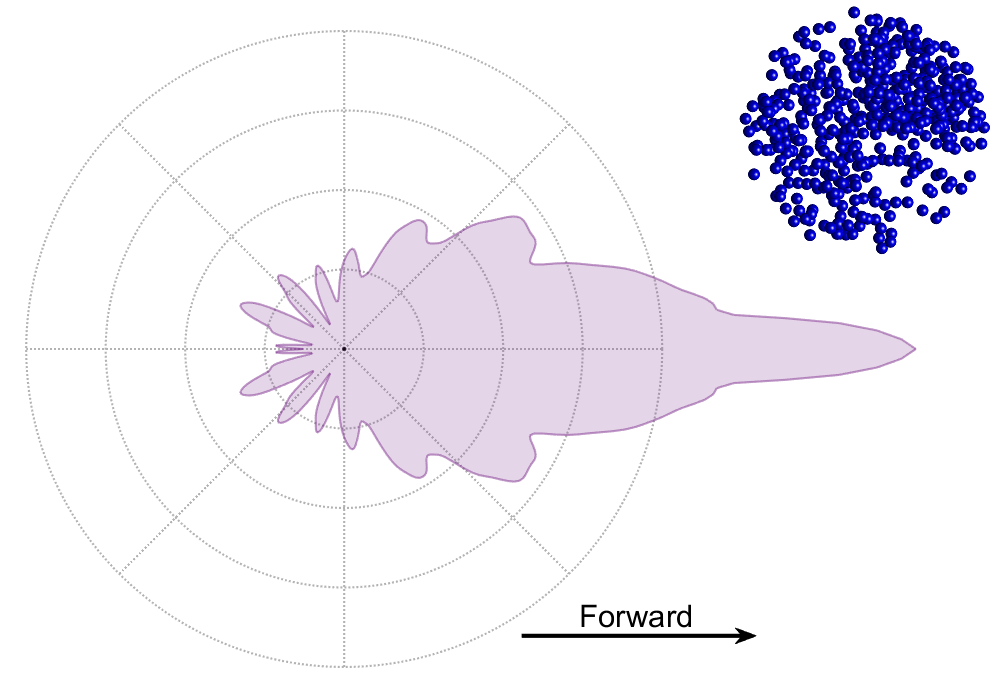
\includegraphics[width=2\resLen]{images/pfunc/negative.png}} & \multicolumn{2}{c}{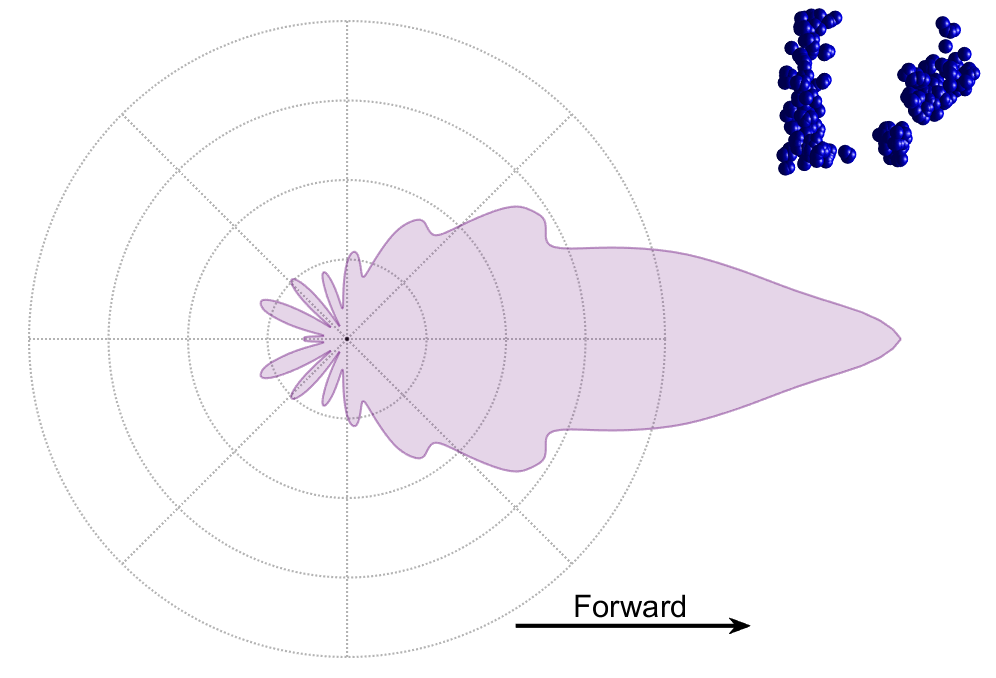
\includegraphics[width=2\resLen]{images/pfunc/positive.png}} 
        \\
        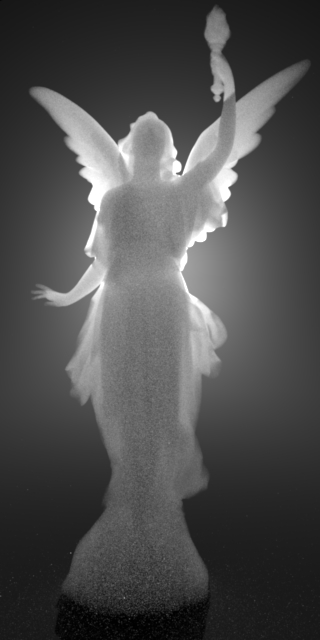
\includegraphics[width=\resLen]{images/lucy/neg_unc.jpg} &
        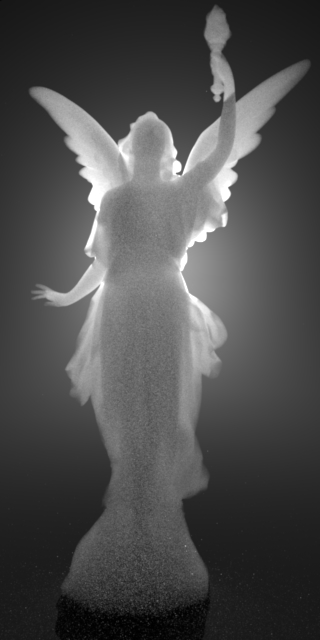
\includegraphics[width=\resLen]{images/lucy/neg_neg.jpg} &
        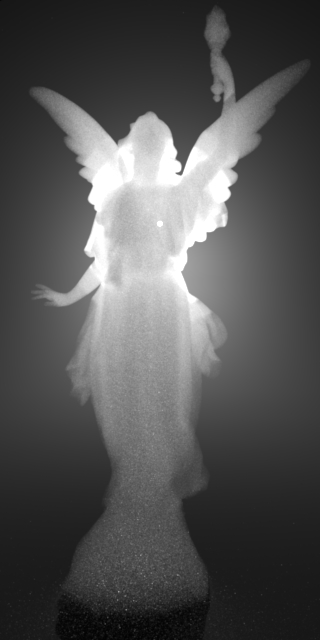
\includegraphics[width=\resLen]{images/lucy/pos_unc.jpg} &
        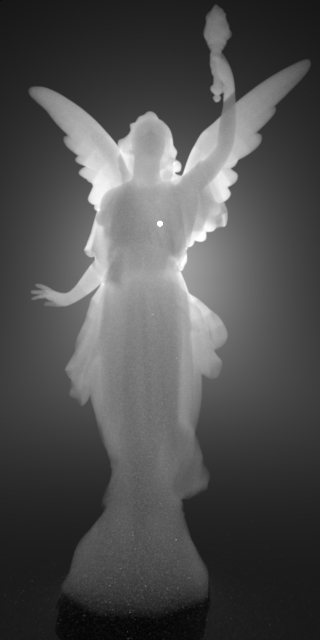
\includegraphics[width=\resLen]{images/lucy/pos_pos.jpg} 
        \\
        (a1) \textbf{unc.} clusters & (a2) \textbf{neg.} clusters & (b1) \textbf{unc.} clusters & (b2) \textbf{pos.} clusters
    \end{tabular}
    \caption{\label{fig:correlated}
        By correlating particle positions negatively (a) or positively (b), our method can produce bulk scattering parameters for near-field correlated media.
        In this example, we use $\lambda = 400\text{nm}$, particle radius~$\radius_i = 500\text{nm}$, and per-cluster particle count $\Ncls = 100$.
        Additionally, we can further correlate particle clusters themselves, a variety of appearances can be achieved (a1--b2).
        (The bright dot in (b1) and (b2) emerges from unscattered light from the area source.)
    }
\end{figure}

